% A LaTeX template for EXECUTIVE SUMMARY of the MSc Thesis submissions to 
% Politecnico di Milano (PoliMi) - School of Industrial and Information Engineering
%
% S. Bonetti, A. Gruttadauria, G. Mescolini, A. Zingaro
% e-mail: template-tesi-ingind@polimi.it
%
% Last Revision: October 2021
%
% Copyright 2021 Politecnico di Milano, Italy. NC-BY

\documentclass[11pt,a4paper,twocolumn]{article}

%------------------------------------------------------------------------------
%	REQUIRED PACKAGES AND  CONFIGURATIONS
%------------------------------------------------------------------------------
% PACKAGES FOR TITLES
\usepackage{titlesec}
\usepackage{color}

% PACKAGES FOR LANGUAGE AND FONT
\usepackage[utf8]{inputenc}
\usepackage[english]{babel}
\usepackage[T1]{fontenc} % Font encoding

% PACKAGES FOR IMAGES
\usepackage{graphicx}
\graphicspath{{Images/}} % Path for images' folder
\usepackage{eso-pic} % For the background picture on the title page
\usepackage{subfig} % Numbered and caption subfigures using \subfloat
\usepackage{caption} % Coloured captions
\usepackage{transparent}

% STANDARD MATH PACKAGES
\usepackage{amsmath}
\usepackage{amsthm}
\usepackage{bm}
\usepackage[overload]{empheq}  % For braced-style systems of equations

% PACKAGES FOR TABLES
\usepackage{tabularx}
\usepackage{longtable} % tables that can span several pages
\usepackage{colortbl}

% PACKAGES FOR ALGORITHMS (PSEUDO-CODE)
\usepackage{algorithm}
\usepackage{algorithmic}

% PACKAGES FOR REFERENCES & BIBLIOGRAPHY
\usepackage[colorlinks=true,linkcolor=black,anchorcolor=black,citecolor=black,filecolor=black,menucolor=black,runcolor=black,urlcolor=black]{hyperref} % Adds clickable links at references
\usepackage{cleveref}
\usepackage[square, numbers, sort&compress]{natbib} % Square brackets, citing references with numbers, citations sorted by appearance in the text and compressed
\bibliographystyle{plain} % You may use a different style adapted to your field

% PACKAGES FOR THE APPENDIX
\usepackage{appendix}

% PACKAGES FOR ITEMIZE & ENUMERATES 
\usepackage{enumitem}

% OTHER PACKAGES
\usepackage{amsthm,thmtools,xcolor} % Coloured "Theorem"
\usepackage{comment} % Comment part of code
\usepackage{fancyhdr} % Fancy headers and footers
\usepackage{lipsum} % Insert dummy text
\usepackage{tcolorbox} % Create coloured boxes (e.g. the one for the key-words)
\usepackage{stfloats} % Correct position of the tables

%-------------------------------------------------------------------------
%	NEW COMMANDS DEFINED
%-------------------------------------------------------------------------
% EXAMPLES OF NEW COMMANDS -> here you see how to define new commands
\newcommand{\bea}{\begin{eqnarray}} % Shortcut for equation arrays
\newcommand{\eea}{\end{eqnarray}}
\newcommand{\e}[1]{\times 10^{#1}}  % Powers of 10 notation
\newcommand{\mathbbm}[1]{\text{\usefont{U}{bbm}{m}{n}#1}} % From mathbbm.sty
\newcommand{\pdev}[2]{\frac{\partial#1}{\partial#2}}
% NB: you can also override some existing commands with the keyword \renewcommand

%----------------------------------------------------------------------------
%	ADD YOUR PACKAGES (be careful of package interaction)
%----------------------------------------------------------------------------


%----------------------------------------------------------------------------
%	ADD YOUR DEFINITIONS AND COMMANDS (be careful of existing commands)
%----------------------------------------------------------------------------


% Do not change Configuration_files/config.tex file unless you really know what you are doing. 
% This file ends the configuration procedures (e.g. customizing commands, definition of new commands)
% Set the geometric layout of the document
\usepackage{geometry}
\geometry{
  top=3cm,
  left = 2.0cm,
  right = 2.0cm,
  bottom=2cm,
  headheight= 2cm,
  headsep= 0cm,
}
\raggedbottom 

% Create color bluePoli (-> manuale grafica coordinata:  https://www.polimi.it/fileadmin/user_upload/il_Politecnico/grafica-coordinata/2015_05_11_46xy_manuale_grafica_coordinata.pdf)
\definecolor{bluePoli}{cmyk}{0.4,0.1,0,0.4}

% Custom theorem environments
\declaretheoremstyle[
  headfont=\color{bluePoli}\normalfont\bfseries,
  bodyfont=\color{black}\normalfont\itshape,
]{colored}

\captionsetup[figure]{labelfont={color=bluePoli}} % Set colour of the captions
\captionsetup[table]{labelfont={color=bluePoli}} % Set colour of the captions
\captionsetup[algorithm]{labelfont={color=bluePoli}} % Set colour of the captions

\theoremstyle{colored}
\newtheorem{theorem}{Theorem}[section]
\newtheorem{proposition}{Proposition}[section]

% Enhances the features of the standard "table" and "tabular" environments.
\newcommand\T{\rule{0pt}{2.6ex}}
\newcommand\B{\rule[-1.2ex]{0pt}{0pt}}

% Algorithm description
\newcounter{algsubstate}
\renewcommand{\thealgsubstate}{\alph{algsubstate}}
\newenvironment{algsubstates}{
    \setcounter{algsubstate}{0}%
    \renewcommand{\STATE}{%
    \stepcounter{algsubstate}%
    \Statex {\small\thealgsubstate:}\space}
    }{}
    
% Custom theorem environment
\newcolumntype{L}[1]{>{\raggedright\let\newline\\\arraybackslash\hspace{0pt}}m{#1}}
\newcolumntype{C}[1]{>{\centering\let\newline\\\arraybackslash\hspace{0pt}}m{#1}}
\newcolumntype{R}[1]{>{\raggedleft\let\newline\\\arraybackslash\hspace{0pt}}m{#1}}

% Custom itemize environment
\setlist[itemize,1]{label=$\bullet$}
\setlist[itemize,2]{label=$\circ$}
\setlist[itemize,3]{label=$-$}
\setlist{nosep}

% Set separation of columns 
\setlength{\columnsep}{30pt}

% Create command for background pic
\newcommand\BackgroundPic{% Adding background picture
	\put(230,358){
		\parbox[b][\paperheight]{\paperwidth}{%
			\vfill
			\centering
			\transparent{0.4}
			
\includegraphics[width=0.5\paperwidth]{raggiera_polimi.eps}%
			\vfill
}}}

% Set indentation
\setlength\parindent{0pt}

% Custom title commands
\titleformat{\section}
{\color{bluePoli}\normalfont\Large\bfseries}
{\color{bluePoli}\thesection.}{1em}{}
\titlespacing*{\section}
{0pt}{2ex}{1ex}

\titleformat{\subsection}
{\color{bluePoli}\normalfont\large\bfseries}
{\color{bluePoli}\thesubsection.}{1em}{}
\titlespacing*{\subsection}
{0pt}{2ex}{1ex}

% Custom headers and footers
\pagestyle{fancy}
\fancyhf{}
      
\fancyfoot{}
\fancyfoot[C]{\thepage} % page
\renewcommand{\headrulewidth}{0mm} % headrule width
\renewcommand{\footrulewidth}{0mm} % footrule width

\makeatletter
\patchcmd{\headrule}{\hrule}{\color{black}\hrule}{}{} % headrule
\patchcmd{\footrule}{\hrule}{\color{black}\hrule}{}{} % footrule
\makeatother

% -> Create the header
\chead[C]{
\centering
\begin{tcolorbox}[arc=0pt, boxrule=0pt, colback=bluePoli!60, width=\textwidth, colupper=white]
    \textbf{Executive summary} \hfill \textbf{\author}  
\end{tcolorbox}
}

% Insert here the info that will be displayed into your Title page 
% -> title of your work
\renewcommand{\title}{Simulating online social media conversations with AI agents calibrated on real-world data}
% -> author name and surname
\renewcommand{\author}{Elisa Composta}
% -> MSc course
\newcommand{\course}{Computer Science and Engineering - Ingegneria Informatica}
% -> advisor name and surname
\newcommand{\advisor}{Prof. Francesco Pierri}
% IF AND ONLY IF you need to modify the co-supervisors you also have to modify the file Configuration_files/title_page.tex (ONLY where it is marked)
\newcommand{\firstcoadvisor}{Nicolò Fontana} % insert if any otherwise comment
\newcommand{\secondcoadvisor}{Francesco Corso} % insert if any otherwise comment
% -> academic year
\newcommand{\YEAR}{2024-2025}

%-------------------------------------------------------------------------
%	BEGIN OF YOUR DOCUMENT
%-------------------------------------------------------------------------
\begin{document}

%-----------------------------------------------------------------------------
% TITLE PAGE
%-----------------------------------------------------------------------------
% DO NOT REMOVE SPACES BETWEEN LINES!

\twocolumn[{\begin{@twocolumnfalse}

\AddToShipoutPicture*{\BackgroundPic}

\hspace{-0.6cm}
\includegraphics[width=0.6\textwidth]{logo_polimi_ing_indinf.eps}

\vspace{-1mm}
\fontsize{0.3cm}{0.5cm}\selectfont \bfseries \textsc{\color{bluePoli} Executive Summary of the Thesis}\\

\vspace{-0.2cm}
\Large{\textbf{\color{bluePoli}{\title}}}\\

\vspace{-0.2cm}
\fontsize{0.3cm}{0.5cm}\selectfont \bfseries \textsc{\color{bluePoli} Laurea Magistrale in \course}\\

\vspace{-0.2cm}
\fontsize{0.3cm}{0.5cm} \selectfont \bfseries Author: \textsc{\textbf{\author}}\\

\vspace{-0.4cm}
\fontsize{0.3cm}{0.5cm}\selectfont \bfseries Advisor: \textsc{\textbf{\advisor}}\\

% if only ONE co-advisor is present:
\vspace{-0.4cm}
\fontsize{0.3cm}{0.5cm}\selectfont \bfseries Co-advisor: \textsc{\textbf{\firstcoadvisor}}\\
% if more than one co-advisors are present:
%\vspace{-0.4cm}
%\fontsize{0.3cm}{0.5cm}\selectfont \bfseries Co-advisors: \textsc{\textbf{\firstcoadvisor}}\textsc{\textbf{\secondcoadvisor}}\\

\vspace{-0.4cm}
\fontsize{0.3cm}{0.5cm}\selectfont \bfseries Academic year: \textsc{\textbf{\YEAR}}

\small \normalfont

\vspace{11pt}

\centerline{\rule{1.0\textwidth}{0.4pt}}

\vspace{15pt}
\end{@twocolumnfalse}}]

\thispagestyle{plain} % In order to not show the header in the first page

%%%%%%%%%%%%%%%%%%%%%%%%%%%%%%
%%     THESIS MAIN TEXT     %%
%%%%%%%%%%%%%%%%%%%%%%%%%%%%%%

\section{Introduction}
\label{sec:introduction}
\section{Related work}
\label{sec:relatedwork}


% ABMs, limitation, LLMs
Many studies have explored the simulation of social dynamics through Agent-Based Modeling (ABM), a widely used approach where complex collective behavior emerges from simple interactions among individuals.
While traditional ABMs are limited by the simplicity of the behavioral rules, recent advancements in Large-Language-Models (LLMs) allow the creation of agents with more realistic and coherent behavior.

% Other studies
Simulations based on LLMs have been used to test different recommendation algorithms, showing for example that promoting the interaction between opposing views can reduce toxicity \cite{törnberg2023evaluate}.
%Some frameworks introduce a memory mechanism \cite{gao2023s3socialnetworksimulationlarge}, enabling agents to to maintain coherence and reproduce realistic attitudinal dynamics.
\textit{Y} \cite{rossetti2024ysocialllmpoweredsocial} is another example of simulation framework, designed as a digital twin of a social media platform, where LLM-based agents can post, reply, react and follow other users, supporting controlled experimentation of online behavior.

% LLM agents and misinformation
\medskip
Rumor dissemination has long existed, even through traditional media, but the raise of online social networks has dramatically increased the speed and scale at which fake news can spread, making it an interesting phenomenon for simulation-based studies.
Traditional ABMs tried to replicate it, but they lacked the complexity of human interactions.
The use of LLM agents, instead, enables the simulation of more realistic dynamics, thanks to their ability to generate realistic and persuasive content, even in the context of disinformation.
Some studies show that both agents' personalities and the underlying network structure influence the disinformation propagation, while other frameworks assign specific roles (e.g., \textit{spreaders}, \textit{verifiers}) to better analyze agent behavior \cite{liu2024tinyslipgiantleap}.

% Opinion Dynamics
\medskip
Another key challenge in social simulations is opinion modeling.
Traditional mathematical models, such as DeGroot or Friedkin-Johnsen, formalize social influence, but simplify the complexity of human communication and interaction.

To overcome these limitations, recent opinion dynamics studies introduced LLM agents, leveraging their ability to role-play and interact through natural language \cite{chuang2024simulatingopiniondynamicsnetworks}. 

This makes them particularly suitable for modeling opinion change in settings where language and social interaction are crucial.


\section{Methods}
\label{sec:methods}

%% Simulation workflow
\subsection{Simulation workflow}
The simulations discussed in this work are based on the Y, framework designed to realistically replicate a social media platform with virtual agents. 

Each simulated day consists of multiple rounds during which a sample of active agents performs actions such as posting and interacting.
Agents start without predefined social connections, allowing the network structure to emerge and evolve over time based on their interactions. 
The system is highly configurable, as it allows to specify parameters such as hourly activity, recommendation algorithms, and agents’ misinformation levels.
In addition to the existing simulator, at the end of each day an additional phase enables agents to update their opinions on the discussed topics.


%% Agents
\subsection{Agents}

One of the biggest challenges in social simulations is to realistically model agents and their behavior. 
This section describes how agents are initialized and modeled, and introduces a new category of agents diffusing misinformation.

% Init
\subsubsection{Initialization}
When creating the population, each agent receives a detailed profile build from a mix of randomly generated features, real-world data, and data sampled from real-world distributions.

Some profile dimensions are randomly sampled: name, surname, email, password and personality.
Personality follows the Big Five model, allowing up to 32 combinations of distinct personalities.
Age and gender are assigned using weighted probabilities based on 2024 Twitter statistics in Italy, restricted to users aged 18-60.

All agents are set with Italian nationality and share four main interests, corresponding to the political topics analyzed in this study: \textit{Civil rights}, \textit{Immigration}, \textit{Nuclear energy}, \textit{Reddito di Cittadinanza}.

To make the users even more realistic and context-aware, some attributes are initialized using real-world data, from a Twitter dataset collected around the 2022 Italian political elections \cite{pierri2023ita}.
This includes the users' political leaning, writing toxicity and activity level.
The activity is normalized in the range $[0,1]$ using a logarithmic transformation to reduce the effect of outliers.

Agents are orchestrated using AutoGen, which enables multi-agent conversations.
Before performing any action, the agents receive a role prompt, specifying its profile, the personal opinions, the supported coalition and their views, and a description of the topics.
The topic descriptions ensure that the agents have the necessary background knowledge on the considered context, and specify the meaning of the stances for each topic.


% Behavior
\subsubsection{Agent's behavior}
When an agent is active, it performs one of the following actions: post a tweet, comment on an existing conversation, or just read a tweet.
The action is selected based on two activity values (in $[0,1]$) that define how likely the agent it to post or comment.
If their sum is less then 1, the remaining probability is automatically assigned to the read action.
This setup helps model user behavior more realistically, using values based on real data.

If the agents writes a post, the topic is randomly picked from the user's interests, among those active in the configured time window.
When the agent comments or reads a post, it can also decide to add a reaction (\textit{like} or \textit{dislike}) and to follow or unfollow the author.
These additional behaviors contribute to shaping the network over time.

To decide which content the agent interacts with, a recommendation system selects the posts to show. Two algorithms are used: \textit{ReverseChronoFollowersPopularity}, that recommends popular recent content mainly from followed users, and \textit{ContentRecSys}, selecting random posts.
For suggesting users to follow, the system \textit{PreferentialAttachment} default algorithm is used, which ranks users according to the product of the agent’s neighbor set size and that of the candidate user.


% Misinfo
\subsubsection{Misinformation Agents}


%% Opinion
\subsection{Opinion modeling and update}
\section{Experiments and discussion}
\label{sec:experiments}

% Experimental setup
The simulations had 100 agents interacting over 21 virtual days, initialized with profiles, personalities and opinions.
The model used is \textit{artifish/llama3.2-uncensored}, available on \textit{Ollama}, chosen for its lack of filters, essential when dealing with political topics or controversial opinions.

Different scenarios were tested by varying two parameters: the level of misinformation (0\%, 5\%, 10\%, and 50\%), and the content recommendation system.
Specifically, two recommender algorithms were used:
\begin{itemize}
    \item \textit{ReverseChronoFollowersPopularity}, which shows recent posts from followed users, with some content from non-followed users to ensure exposure to different views
    \item \textit{ContentRecSys}, suggesting random content
\end{itemize}

Each scenario was run 10 to 20 times with new agents, to ensure the robustness of the results.



% Results and discussion
\medskip
The analysis is structured on multiple levels to provide a overview of the behavior of LLMs agents within a simulated social media.

% Interactions
\subsection{Interactions}

% Activity per user type + network structure
The comparison of interaction activity by user type, in Figure \ref{fig:interactions_count}, shows that misinformation agents are more active in content generation, as they post and comment more than base users. However, they engage less in building connections, as \textit{follows} are significantly lower.
\textit{Likes} are used similarly by the two groups, while base users are more active in expressing disagreement through \textit{dislikes}.
Thanks to the \textit{follow} action, users form connections across coalitions and between different agent types, allowing a structured network to emerge. The \textit{unfollow} action, instead, is almost absent, suggesting that longer simulations may be needed to see a observe the evolution of the connections over time.

\begin{figure}[h]
    \centering
    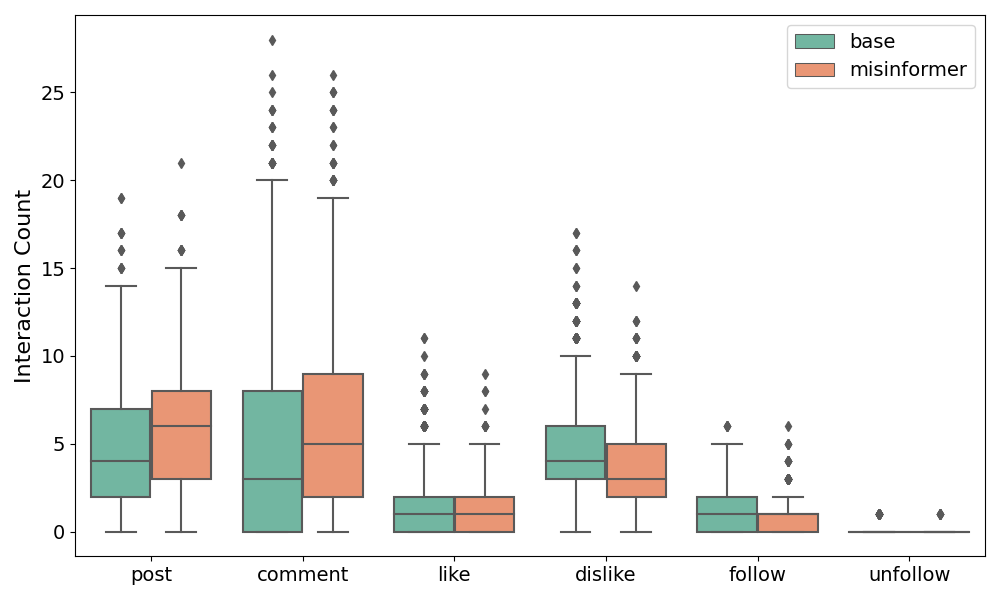
\includegraphics[width=1\linewidth]{Images/Interactions/count_per_user_DefaultRecSys.png}
    \caption{Number of interactions per user by agent type, with each point representing a single user from a simulation run.}
    \label{fig:interactions_count}
\end{figure}

% In-group and out-group interactions across coalitions
\medskip
To analyze how users interact within and across coalitions, Figure \ref{fig:interactions_inout} shows, for each coalition, the percentage of in-group interactions, categorizing the actions into positive (\textit{like}, \textit{follow}) and negative (\textit{dislike}, \textit{unfollow}).

Looking at positive interactions, Centre-Left and Third Pole show a balanced behavior, with about a half of their \textit{likes} and \textit{follows} directed at in-group users.
In contrast, M5S and Right show fewer in-group positive interactions. 
For M5S, this may be due to its smaller size in the simulated populations, which increases the chance of out-group interactions.
The Right, even though it's one of the largest group, still shows a strong preference for out-group positive interactions.

Negative interactions are mostly directed toward other coalitions, and the Right stands out for the higher rate of in-group negative interactions.
This might indicate that the Right may have a greater level of internal fragmentation, with more conflict among users, even if sharing the same political views.

\begin{figure}[h]
    \centering
    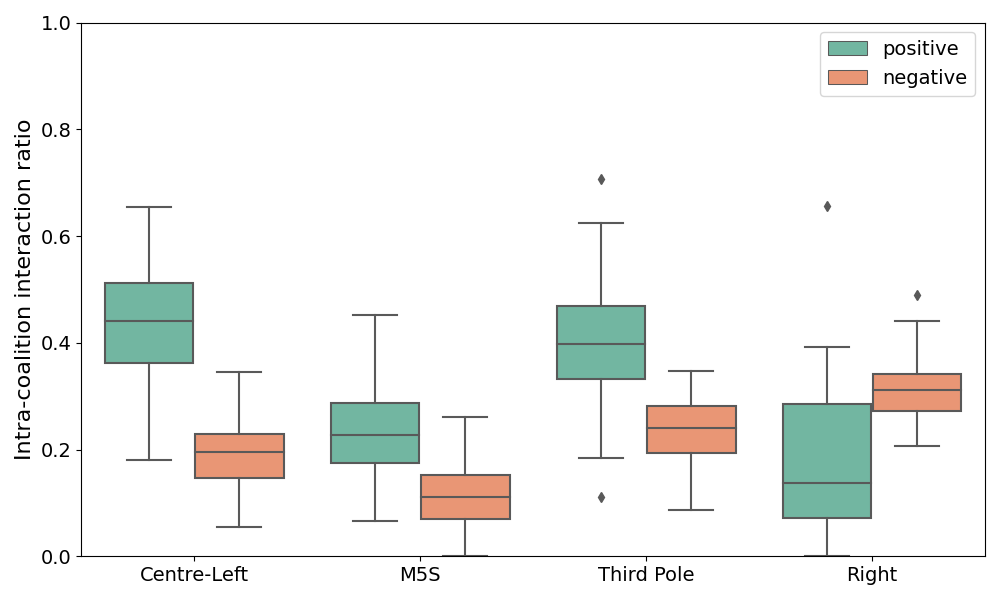
\includegraphics[width=1\linewidth]{Images/Interactions/pos_neg_in_DefaultRecSys.png}
    \caption{Percentage of in-group interactions, divided into positive and negative interactions, for each coalition, with each point representing the ratio from a single simulation run.}
    \label{fig:interactions_inout}
\end{figure}


% Opinion
\subsection{Opinion evolution}
One important aspect introduced in this work in extension to the existing simulator is opinion modeling.
Figure \ref{fig:opinion_evolution} shows that the opinion evolution of scores assigned by LLMs have the same trends as traditional opinion dynamics models.
This confirms that LLMs can effectively model opinion change at population level.
Coalitions that start with the same opinion tend to evolve in parallel, suggesting that their initial view is more influential than the coalition itself.
Moreover, across all topics, there's a gradual convergence toward neutral values, indicating a general reduction in polarization over time.


\begin{figure}[h]
    \centering
    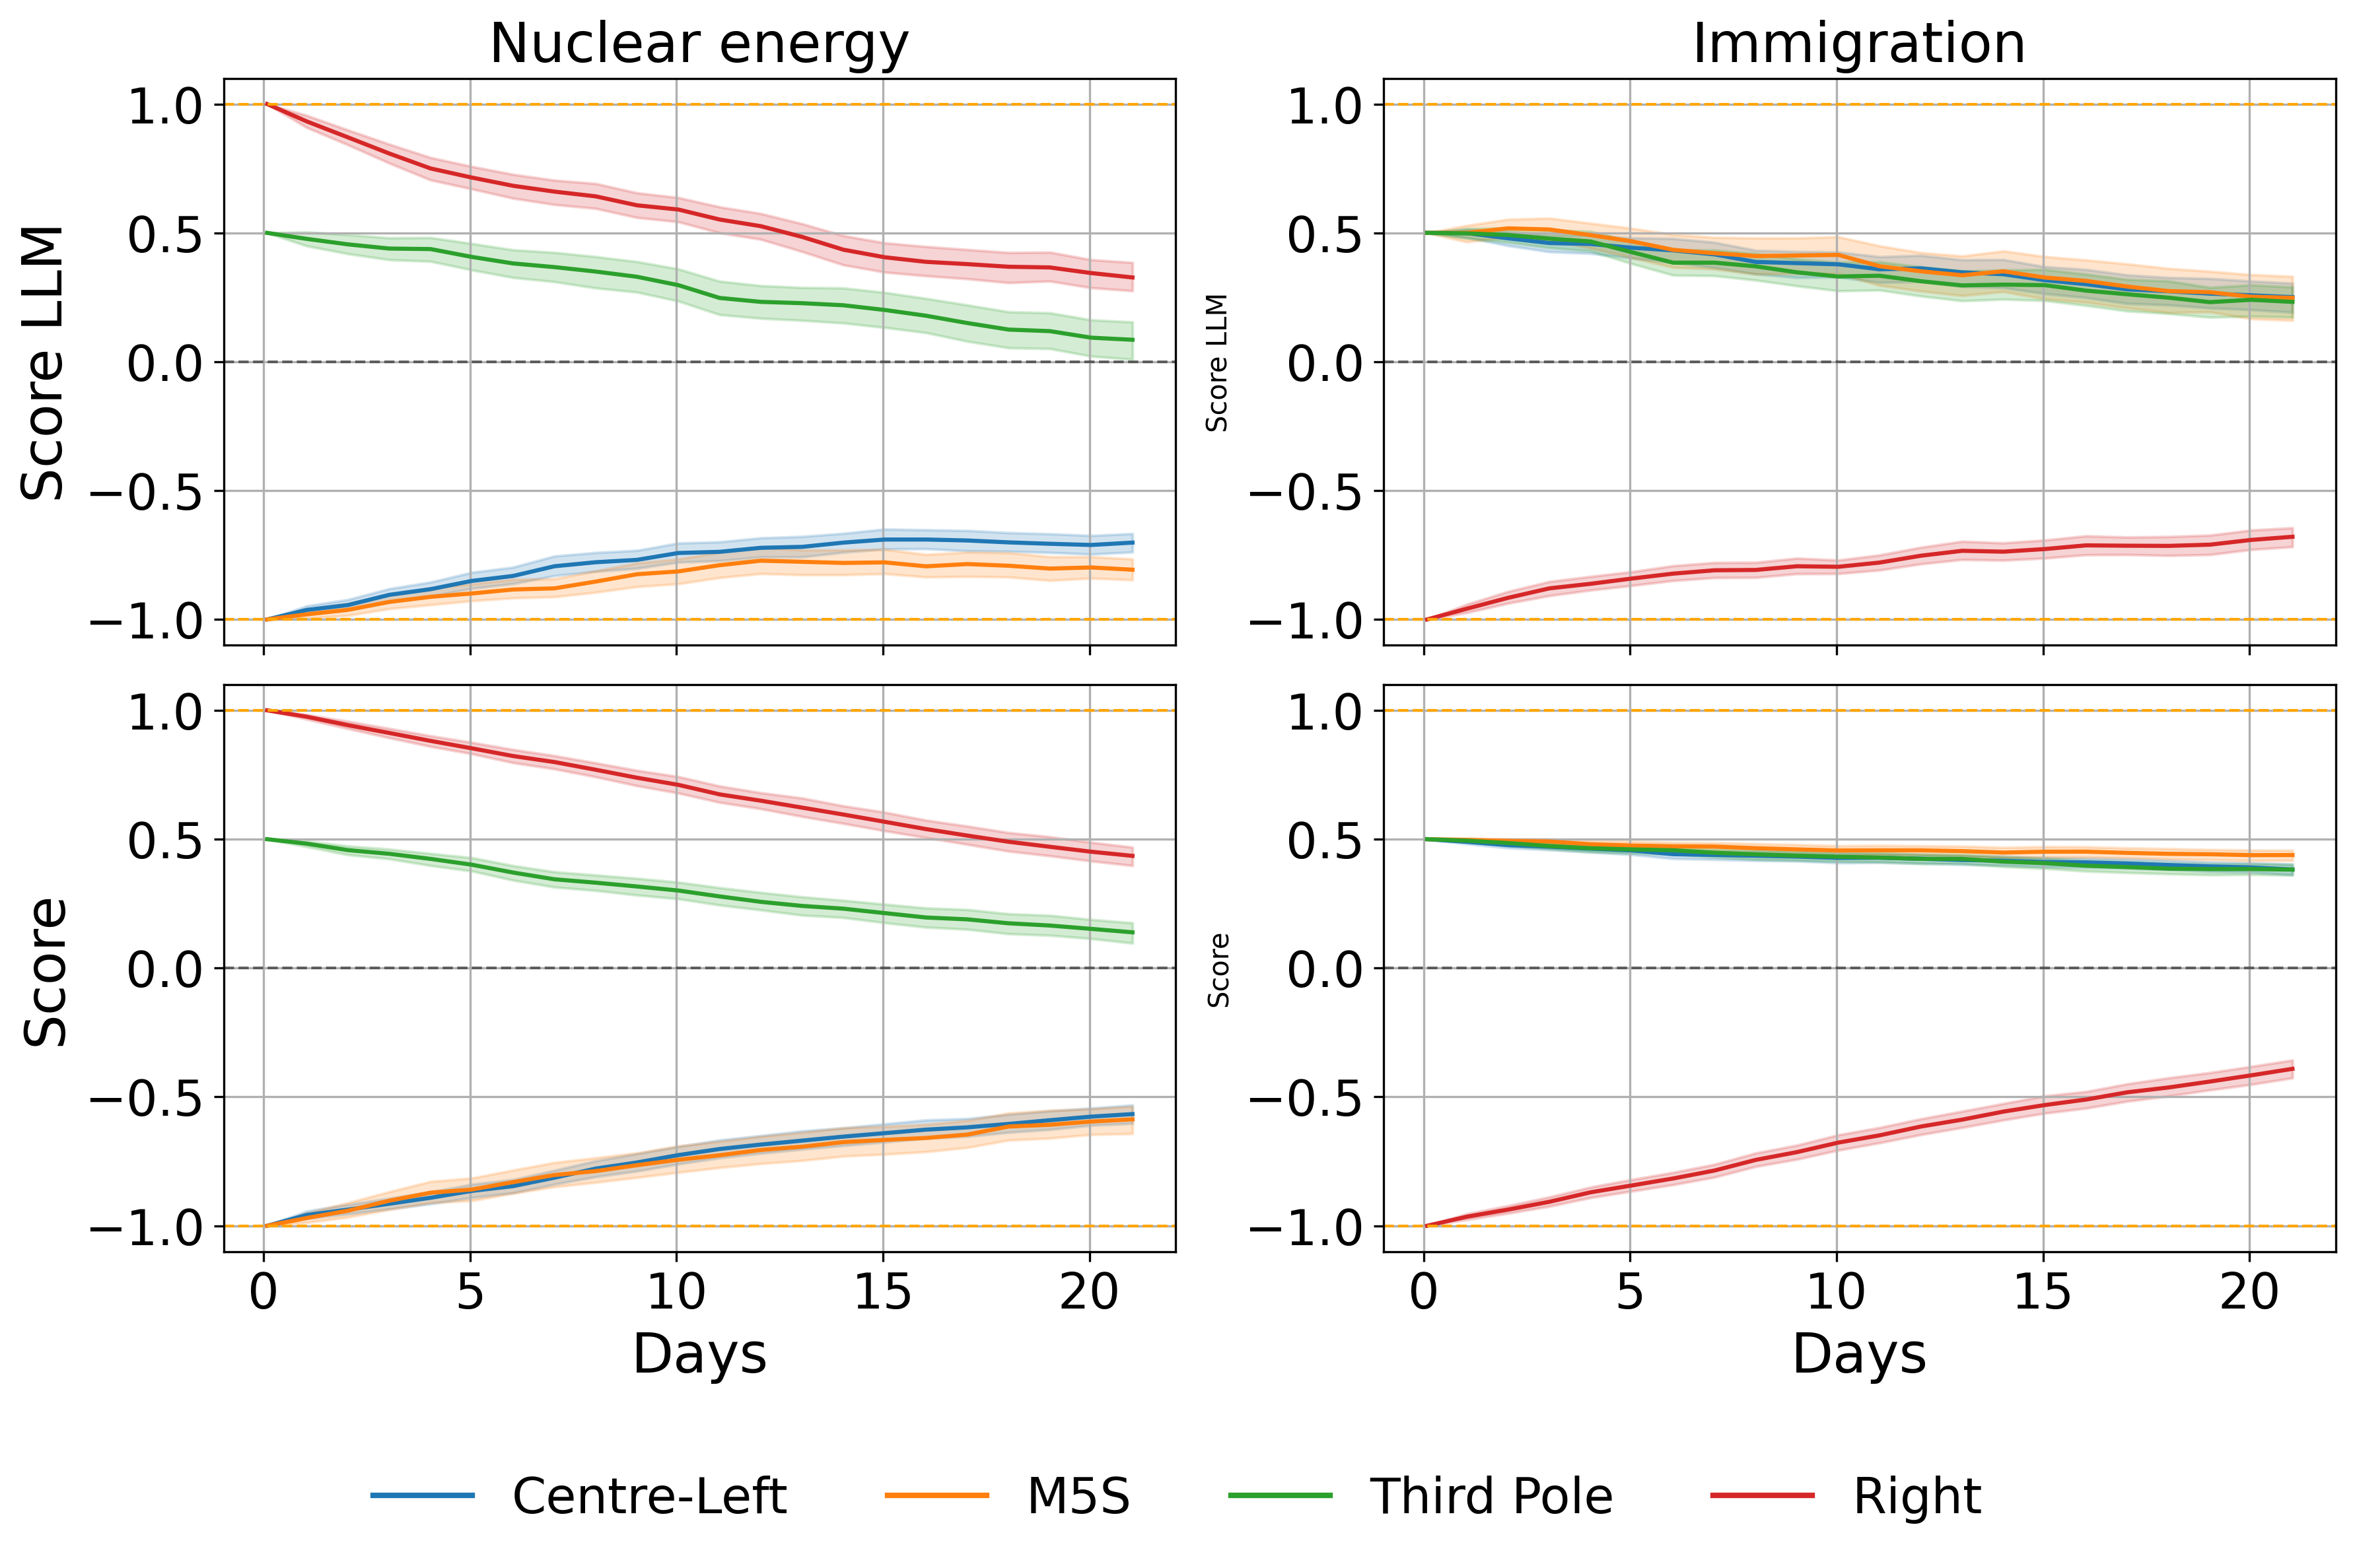
\includegraphics[width=1\linewidth]{Images/Opinions/d21a100m00x_RandomRecSys.png}
    \caption{Opinion evolution, with scores assigned by the LLM and a traditional model, aggregated across all simulation runs of a single experimental setup.}
    \label{fig:opinion_evolution}
\end{figure}


% Misinformation
\subsection{Misinformation}
To evaluate the impact of misinformation, we considered opinion shift, which is the difference between each user’s final and initial opinion.
Results in Figure \ref{fig:misinfo_opinion_shift} show that increasing the amount of misinformation in the system doesn’t significantly affect how agents update their views.
Even in the extreme scenario with 50\% of agents producing misleading content, opinion shifts remains similar to those in setups with lower misinformation.

% Confirmation bias
A possible question is whether the lack of misinformation impact might be related to the confirmation bias, which was explicitly introduced in this work.
While the bias is visible, in the narrow distributions indicating a resistance to opinion change, it affects all conditions equally, and doesn't explain the absence of differences across misinformation levels.
Agents do evolve their opinions over time, but the dynamics of change are independent from the misinformation exposure.

% Coalitions
%A comparison between different coalitions highlights that the Right has the narrowest distributions, suggesting greater resistant to change.
%This may be due to their stronger initial stances, both in the numerical scores and in the descriptions of their view, which led agents to remain closer to their starting position.

% Conclusion on LLM limitation
These findings reveal a limitation: even though LLMs can simulate realistic opinion change, they don't replicate the real-world susceptibility to misinformation.
This may be due to missing factors such as emotional reasoning or social signals such as popularity or perceived credibility.
Adding these factors could improve future simulations.


\begin{figure}[h]
    \centering
    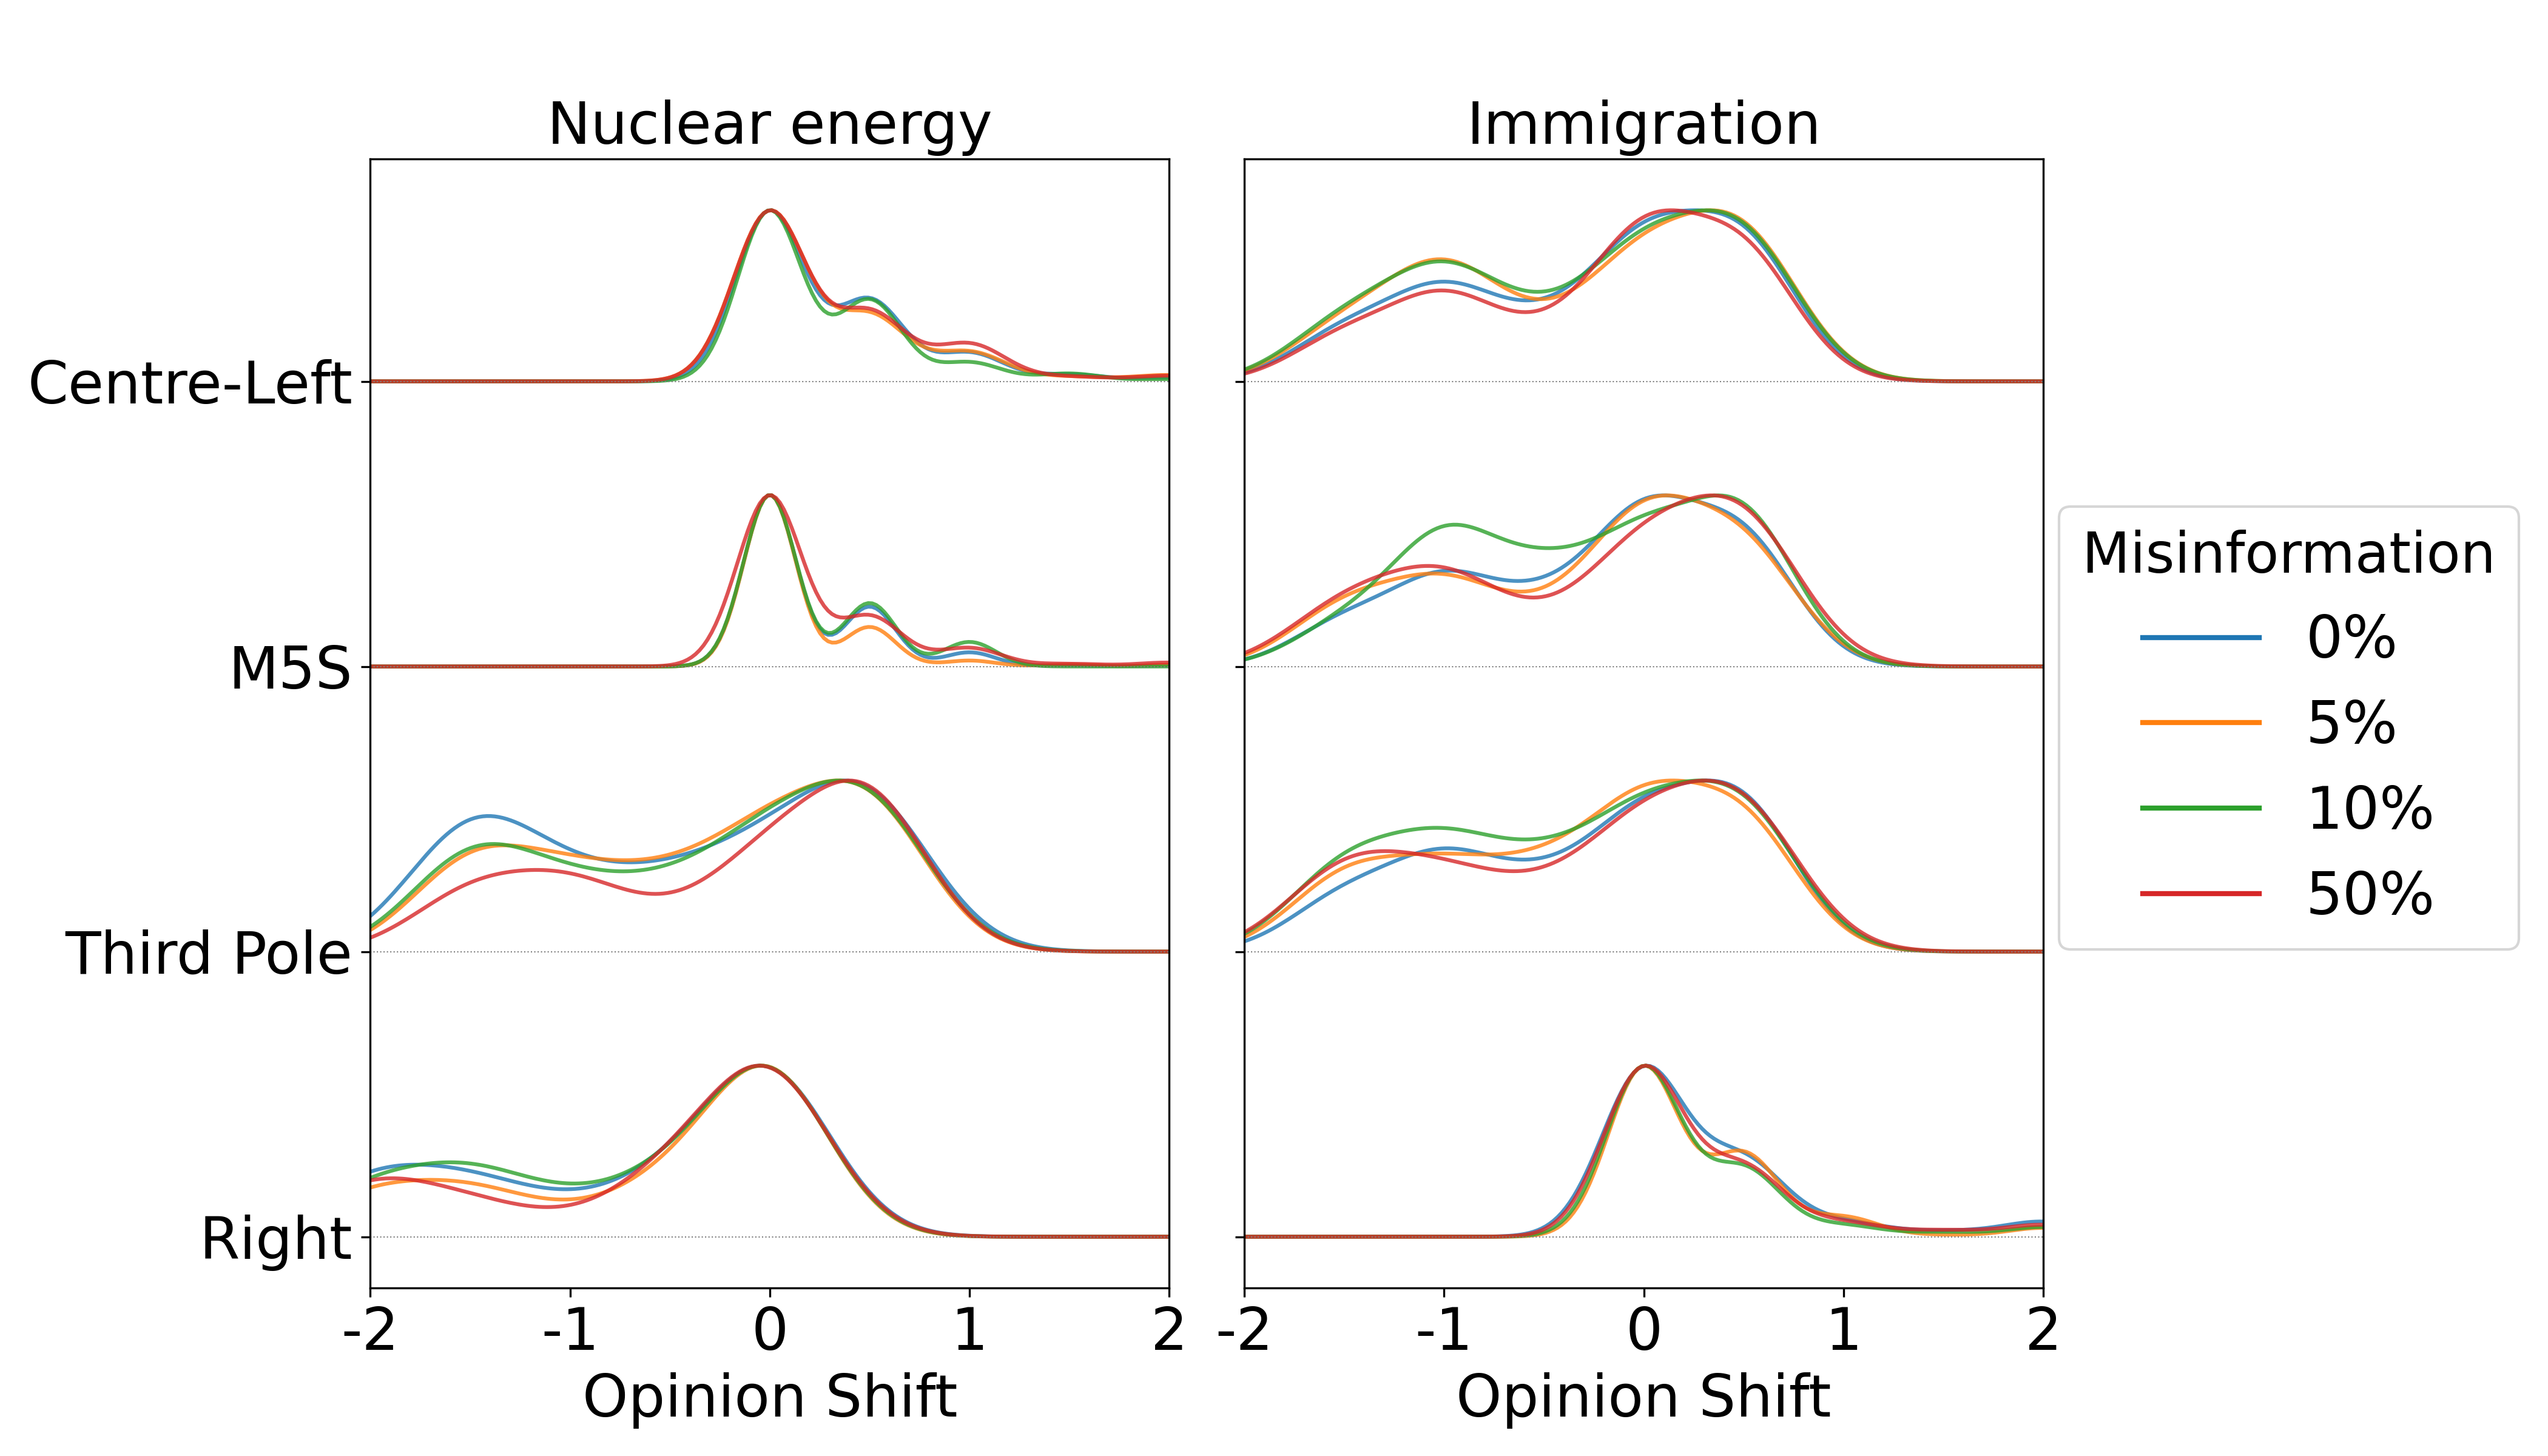
\includegraphics[width=1\linewidth]{Images/Misinformation/score_llm_RandomRecSys_small.png}
    \caption{Distribution of individual users’ opinion shifts by topic and coalition across all simulation runs for each misinformation level.}
    \label{fig:misinfo_opinion_shift}
\end{figure}


% Toxicity
\subsection{Toxicity analysis}

% Toward in-group and out-group 
To evaluate how agents express toxicity toward different groups, we compute the delta of the logarithms of the toxicity of comments directed to out-group and in-group users.
Figure \ref{fig:toxicity_in_out} shows that both real and simulated data are centered around zero, indicating that agents don't have a specific preference in toxicity direction.

However, the real data have a wider distribution, indicating that real users show greater variability in the toxicity toward the two groups.
This suggests that the simulations fail to reproduce the diversity of behavior of real world  in how toxicity is distributed.



\begin{figure}[h]
    \centering
    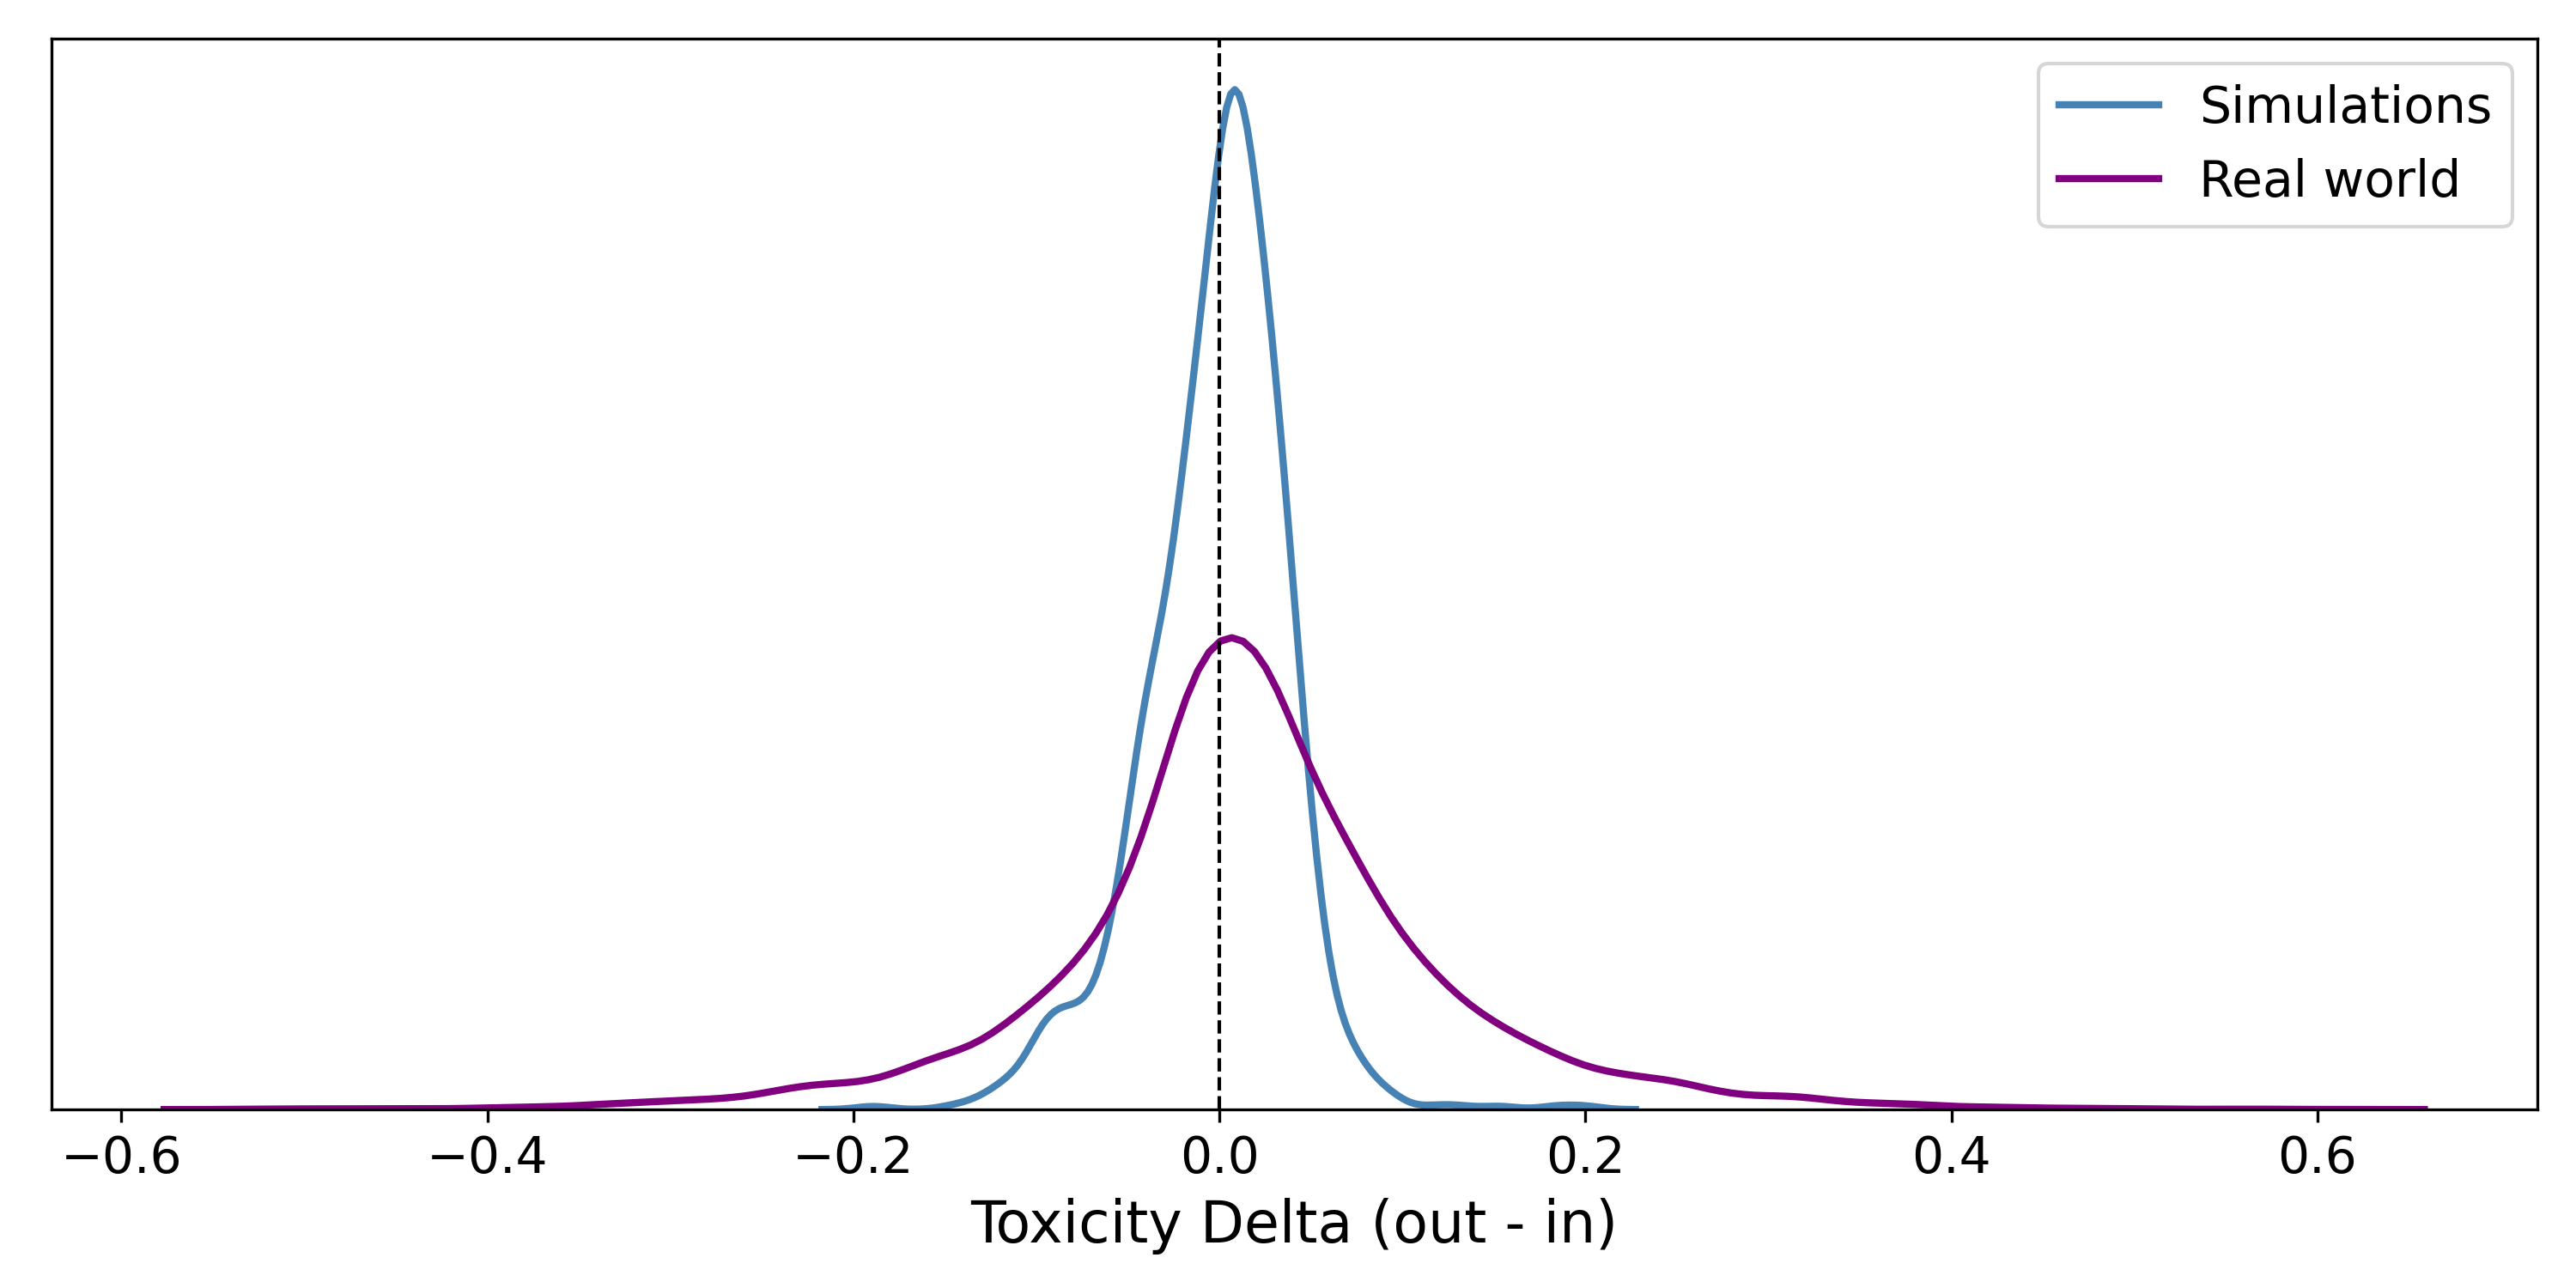
\includegraphics[width=1\linewidth]{Images/Toxicity/diff_in_out_combined.png}
    \caption{Distribution of the difference in mean toxicity toward out-group and in-group comments for each user in each simulation.}
    \label{fig:toxicity_in_out}
\end{figure}


% Across coalitions and content types
\medskip
Figure \ref{fig:toxicity_box} investigates how toxicity varies across political coalition and content types.

In general, posts tend to be more toxic than comments, except for the Right coalition, which may indicate a more conflictual style in replying.
M5S has the highest average toxicity in posts, whereas Centre-Left and Third Pole maintain a more moderate and stable tone in both types of contents.

Despite the low average values, all distributions have a positive skew, suggesting that LLMs can produce highly toxic content, even though at lower frequency.
This behavior, possibly facilitated by the use of an uncensored model, contributes to a more realistic simulation of online conversations.


\begin{figure}[h]
    \centering
    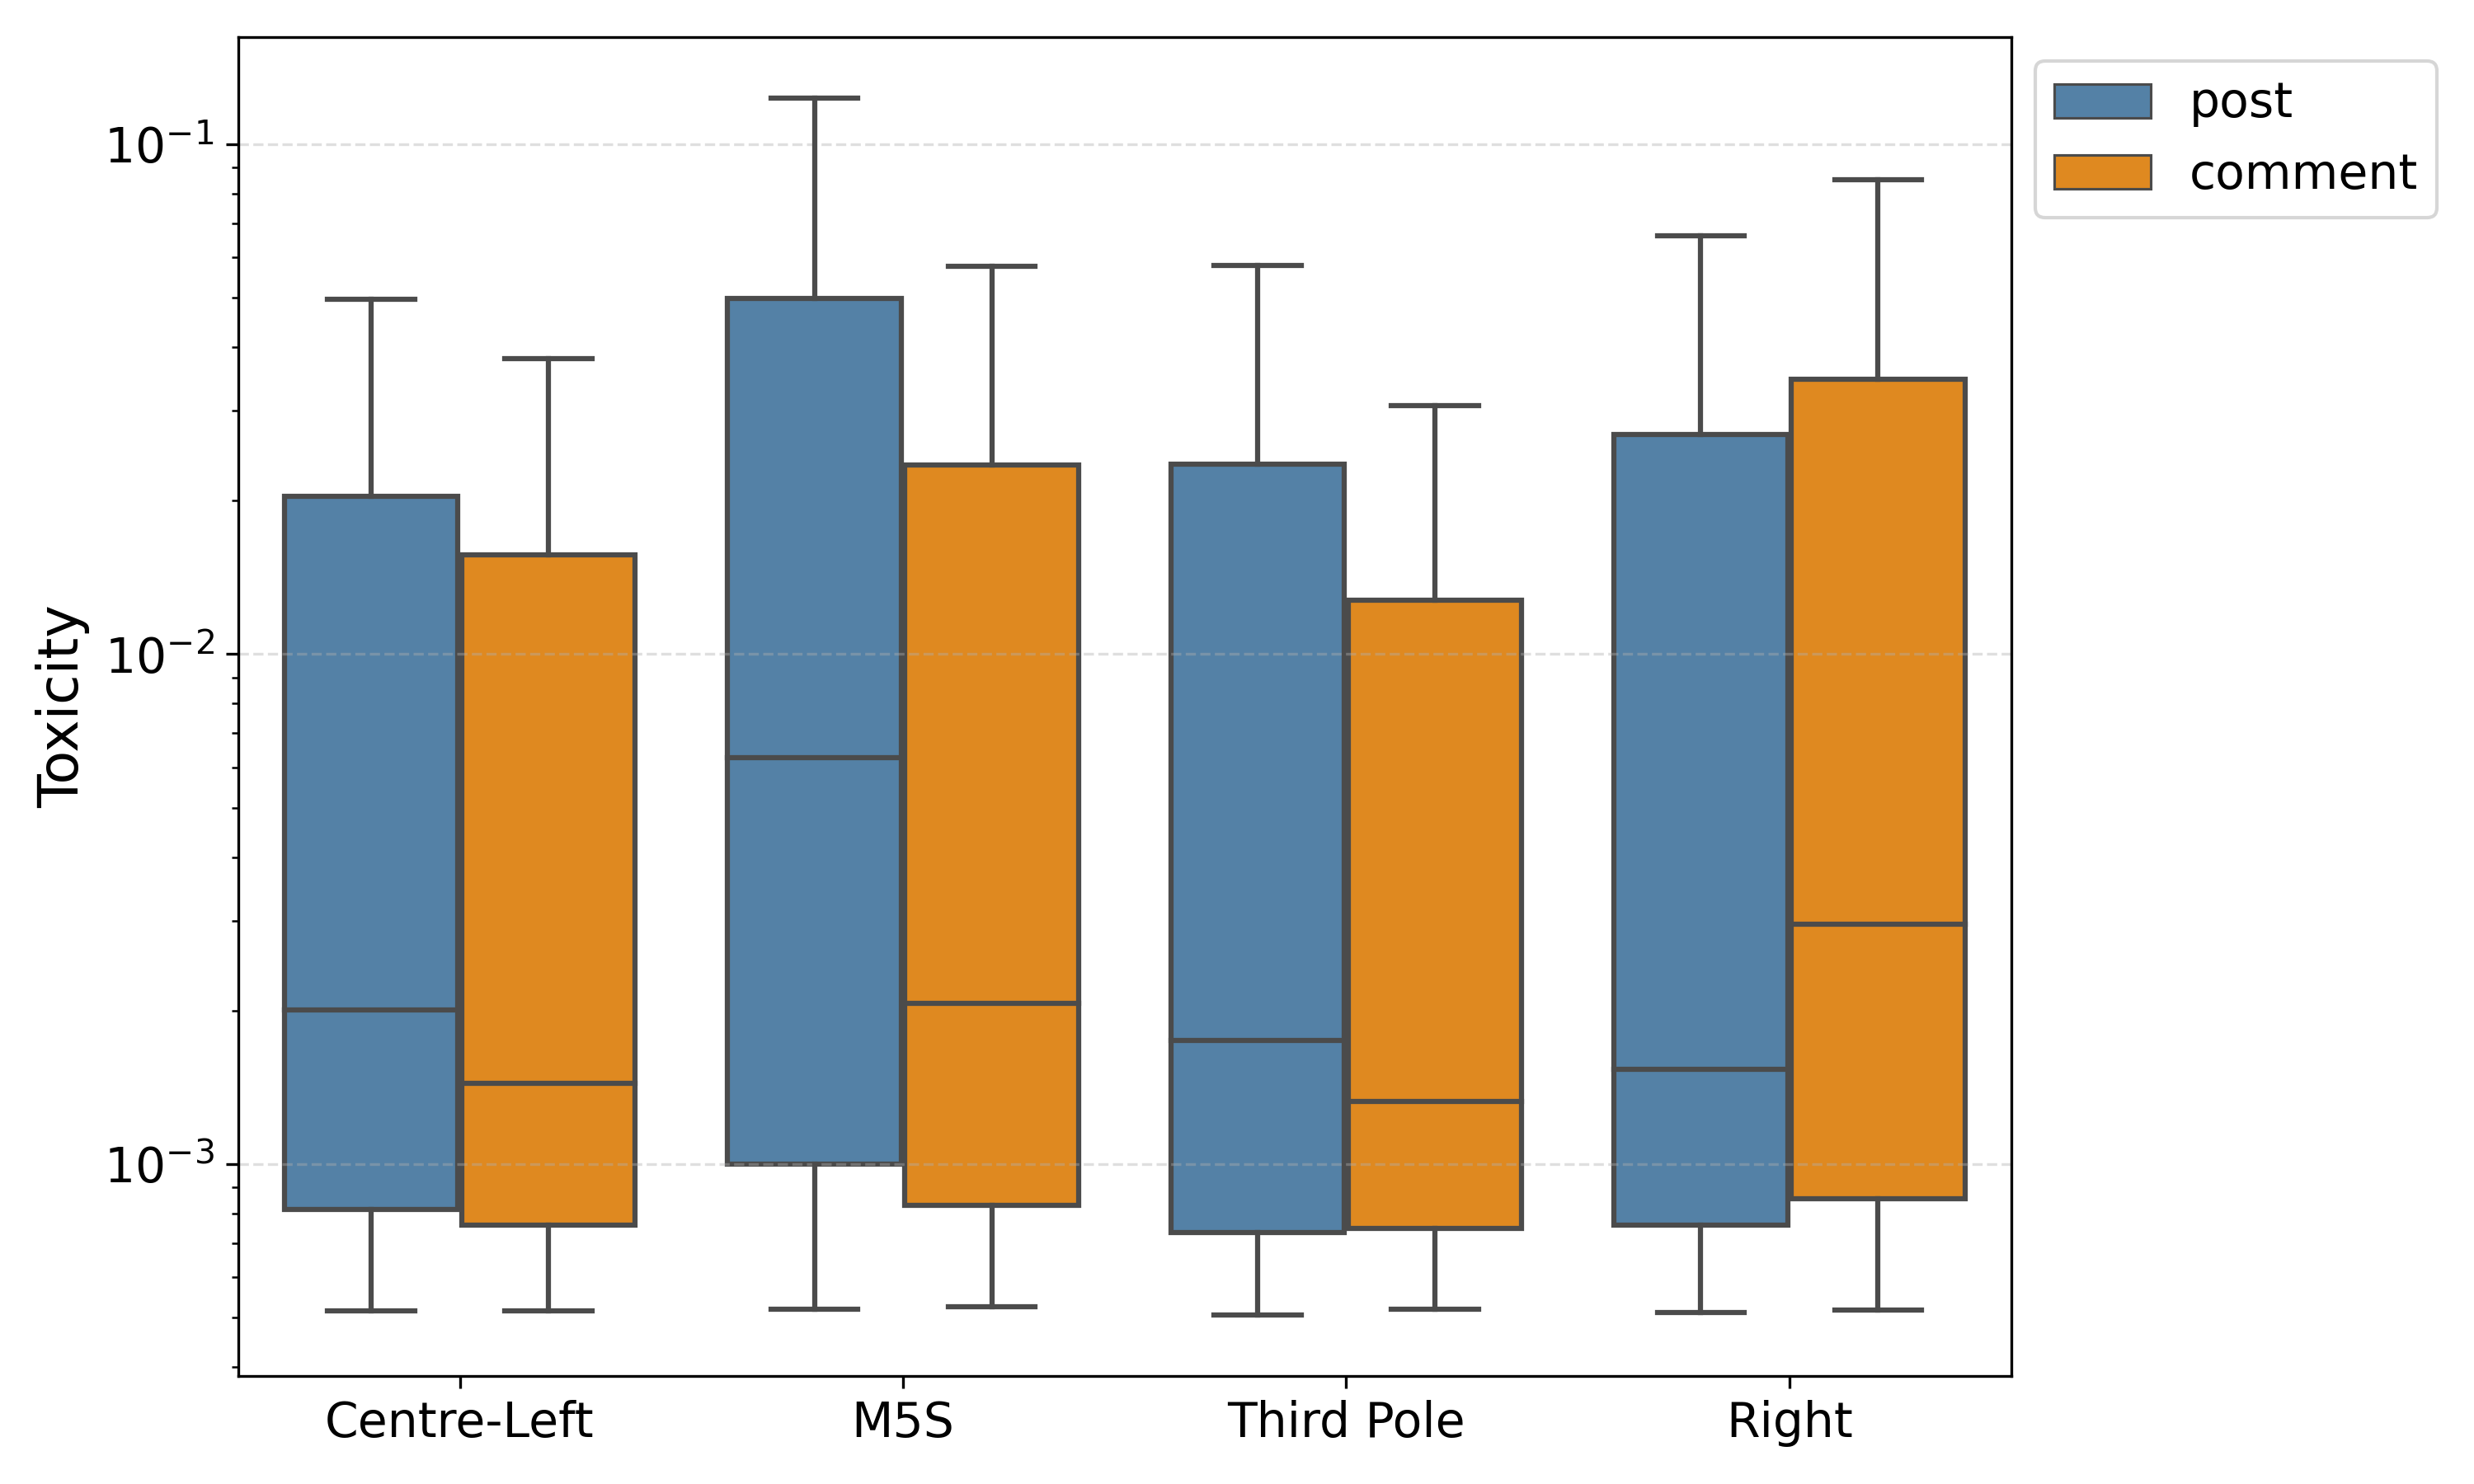
\includegraphics[width=1\linewidth]{Images/Toxicity/box_posts_vs_comments.png}
    \caption{Toxicity of LLM-generated texts by political coalition, including all posts and comments from all simulations.}
    \label{fig:toxicity_box}
\end{figure}


\subsection{Content recommendations}
The comparison on the two content recommendation algorithms doesn't reveal any significant behavioral difference.
At the beginning of the simulation, agents are not yet connected, so the default algorithm, \textit{ReverseChronoFollowersPopularity}, doesn't have follower information, and ends up behaving as the random recommender, \textit{ContentRecSys}.

As shown in Figure \ref{fig:recsys_comparison}, both the volume and the in-group ration of interactions is similar across the two algorithms.
To observe more meaningful effects, simulations should either run for a longer virtual time or start from a network with preexisting connections, allowing the recommender system to have a greater influence.


\begin{figure}[h]
    \centering
    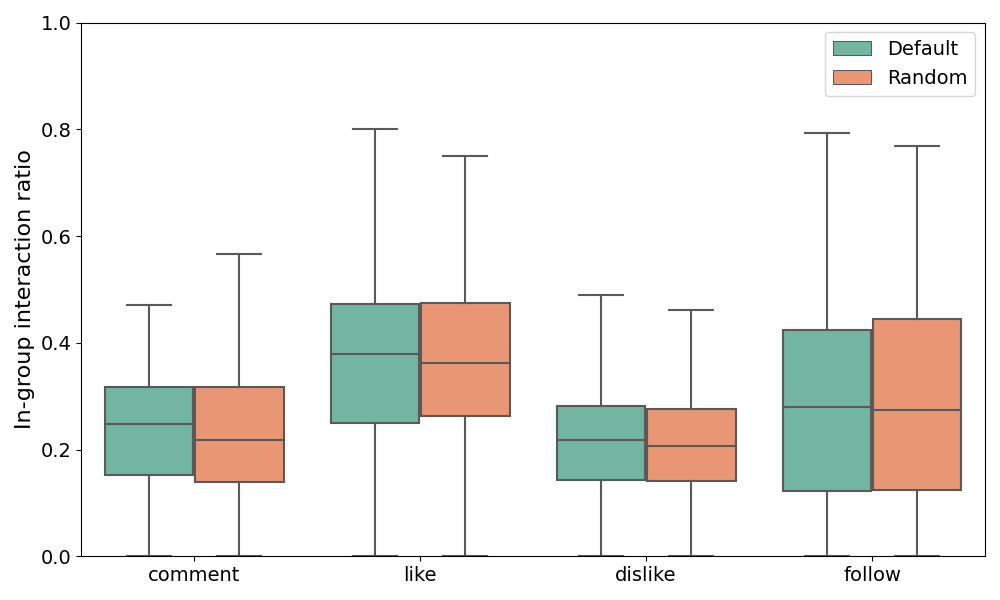
\includegraphics[width=1\linewidth]{Images/Recsys/recsys_in_group_ratio.png}
    \caption{Percentage of in-group interactions by type for two recommendation algorithms, with each point representing a single simulation run.}
    \label{fig:recsys_comparison}
\end{figure}
\section{Conclusions}
\label{sec:conclusion}

% Intro
This work explored the use of LLMs as agents in social simulations.
The original \textit{Y} simulator was extended to integrate opinion modeling, misinformation agents, and a realistic initialization based on real-world data.

% Main results
The simulations showed that LLM-based agents are capable of interacting, generating content with different linguistic styles, and forming social connections. 
Opinion scores assigned by LLMs followed trends similar to those of traditional opinion dynamics models, supporting their validity for population-level analysis.

% Limitations
However, some limitations emerged.
First, the duration of the simulations (21 virtual days) was not sufficient to observe long-term effects.
For example, the impact of different content recommendation systems didn't emerge, as the network was not yet sufficiently structured in the first virtual days. 
Another limitation is that agents, despite being enriched with personality traits and confirmation bias, lacked some cognitive and emotional mechanisms necessary to reproduce real-world dynamics, such as the susceptibility to misinformation, which resulted negligible in the simulations.

% Future work
Future research could explore a wider range of disinformation strategies (e.g., bots, coordinated groups), integrate multimodal content (text, images, videos), or introduce external events during the simulation timeline. 
Additionally, a comparison of the simulation results with real-world data would help assess the realism of the emergent behaviors and validate LLM-based agents.

% Conclusion
Overall, this work shows that LLMs are a powerful tool for simulating complex social phenomena, enabling more realistic modeling of language and interaction in agent-based systems.
However, replicating complex human traits, such as emotional reasoning and susceptibility to manipulation, remains a challenge.
Further studies are required to make these simulations closer to real-world dynamics by capturing deeper individual and social factors.



\section*{Acknowledgements}
Here you might want to acknowledge someone.

\bibliography{bibliography.bib} 

\end{document}